\documentclass[12pt]{article}
%\input{hw_macros.tex}

\setlength{\topmargin}{-.75in} \addtolength{\textheight}{2.00in}
\setlength{\oddsidemargin}{.00in} \addtolength{\textwidth}{.75in}

\usepackage{amsmath,color,amssymb,graphicx,esdiff}
\usepackage[shortlabels]{enumitem}
\pagestyle{empty}
\usepackage{listings}

\setlength{\parindent}{0in}
\setlist[enumerate]{leftmargin=*}
\begin{document}

{\sc {\bf {\large Homework 4}}
            \hfill {MTH 629, Fall 2021}}
\bigskip

{\bf Due Tuesday, Nov. 23\textsuperscript{th} by 11:59 pm on Canvas}

A medical lab is testing machine learning software which actively regulates oxygen levels in ventilators. If oxygen levels fall outside of an acceptable range, the ventilators automatically reset. A twenty day study is done with the response variable the time in days (eventtime) until the ventilators reset. The exposure variable, Setting, indicates whether the software is disabled (Setting=2), at the standard setting (Setting=1) or at the newly coded setting (Setting=0). The variable LO2 indicates the level of oxygen gas, compared to a baseline, that is supplied to the ventilator through a main tube. In addition, the Ventilators are from two different manufacturers, Philips (Mft=0) and Hamilton Medical (Mft=1).


\section{Chapter 5}

\begin{enumerate}[1.]
\item Load the data by using the following command in R: \\
 \lstinline{Ven.reset <-read.csv(``Venreset.csv'', header = TRUE)}

\item Test the proportional hazard (PH) assumption for the variables Setting, LO2 and Mft:
\begin{enumerate}[i.]
\item Use a GOF test using Schoenfeld Residuals to test each variable. Conduct your test at significance level $\alpha=0.05$.
\item From homework 3 we saw that Setting and LO2 satisfy the PH assumption.  Test whether MFT satisfies the PH assumption by using the alternative approach to log-log plots (as in problem 4.2 in the slides). For your adjusted survival curves, use the overall mean of LO2 and the overall mean of Setting. Add a legend to your log-log plots.
\item What conclusion do you reach from the Schoenfeld residuals and from your adjusted log-log plots about the covariate Mft and the PH assumption?
\end{enumerate}
\item Fitting and examining a stratified Cox PH model without interaction.
\begin{enumerate}[i.]
\item Fit a stratified Cox PH model to the Ventilator Reset data without interaction. Use Setting and LO2 as covariates and stratify on Mft. Give your fitted stratified model.
\item Use individual Wald tests to test for the significance of Setting and LO2 at $\alpha=0.05$.
\item Use a Likelihood ratio test to test for the overall significance of Setting and LO2 at $\alpha=0.05$. 
\item Interpret the coefficients of Setting and LO2 in the stratified Cox PH model. 
\item Plot the adjusted survival curves for Setting from your stratified Cox PH model. Set LO2=mean(LO2). Do the curves suggest significant interaction between Setting and Mft adjusted for LO2?
\end{enumerate}
\vspace{30pt}

\item Fitting and examining a stratified Cox PH model with interaction.
\begin{enumerate}[i.]
\item Fit a stratified Cox PH model to the Ventilator Reset Data. Use Setting and LO2 as covariates and stratify on Mft. Assume interaction of the covariates with Mft.
\item Test the interaction assumption using a likelihood ratio test at significance level $\alpha=0.05$.
\item Using the interaction model, find the HR of Setting for Mft=0 and Mft=1 (take into account interaction). Also, find the $95\%$ CI's of these HR's. Do the CI's for these HR's overlap? Does this agree with a Wald test of the interaction term between Setting and Mft?
\end{enumerate}
\item The dataset Mayothtcancer.dat considers survival times of 265 throat cancer patients from the Mayo cancer clinic in Rochester, MN. The data set has six variables listed as follows:
\begin{enumerate}[ ]
\item $X_1:$ 1 if cancer type is Nasopharynx, 0 otherwise
\item $X_2:$ 1 if cancer type is Oropharynx, 0 otherwise
\item $X_3:$ 1 if cancer type is Hypopharynx, 0 otherwise
\item $X_4:$ BMI score (18.5 - 39.9)
\item $X_5:$ Age (22-87)
\item $X_6:$  0 if chemotherapy and 1 if surgery.
\end{enumerate}
A GOF test using Schoenfeld Residulas and graphical tests suggest $X_4, X_5$ and $X_6$ satisfy the PH assumption and $X_1,X_2$ and $X_3$ do not. A survival object, $W$, for the survival times is created and a model stratified on the three cancer types is fit. The (partial) results of fitting the model are as follows:
\begin{center}
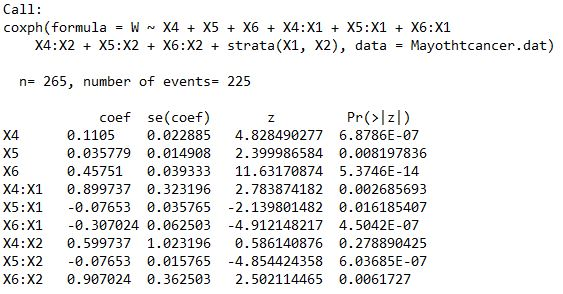
\includegraphics[scale=.9]{HW4_Q5.JPG}
\end{center}
Mr. Brown has an age of 35 and a BMI of 25. Mr. Jones has an age of 50 and a BMI of 29.5. Using the fitted model, give the HR for chemotherapy vs surgery for both patients if:
\begin{enumerate}
\item  the patient has Nasopharynx throat cancer.
\item  the patient has Oropharynx throat cancer.
\item  the patient has Hypopharynx throat cancer.
\end{enumerate}
\item A small study is conducted to test the effectiveness of a medication to treat alcohol dependence. The exposure variable is Dose in mg with 0 indicating the subject receives a placebo.  A extra medication type variable is included which is known not to satisfy the PH assumption.  The response is time in weeks until alcohol consumption. The data below is collected on 7 subjects. Assuming no interaction, create an appropriate SC model for this data and estimate the parameters by maximizing the partial likelihood.
\begin{center}
\begin{tabular}{ c c c c c} \hline
Subject & Time & Status & Dose & Type \\ \hline
1 & 2 & 1 &  0 & 0\\
 2 & 3 & 1 &  2 & 0\\
3 & 5 & 0  & 1 & 1\\
4  & 6 & 1  & 1 & 1\\
5  & 6 & 0  & 1.5 & 0 \\
6  & 7 & 1  & 2 & 1 \\
7  & 8 & 1  & 1.5 & 0 \\
\end{tabular}
\end{center}
Fit a stratified Cox PH model to the data. Your estimate of $\beta$ should be similar to the one you got in your optimization routine (the same sign and within 0.16 of each other). 
According to your estimate, what is the effect of a unit increase of Dose on the hazard (the HR), regardless of type (use either estimate)? 
\end{enumerate} 


\section{Chapter 6}
In the previous chapter, in the Ventilator data set, Mft didn't satisfy the PH assumption but Setting and LO2 did. Thus, we fit a stratified model Cox PH, stratifying on Mft with Setting and LO2 as covariates. We are now going to test Mft for the PH assumption using defined time-dependent covariates in an extended Cox PH model. We are also going to model Mft  in an extended Cox PH model, so that we can get a (time-dependent) HR for this variable.
\begin{enumerate}
\item Create adjusted survival curves for Mft with Setting and LO2 in the model. Use the means of LO2 and setting for your two adjusted survival curves with Mft=0 and Mft=1, respectively.  
\item Based on your adjusted survival curves, choose a ``split point'' for the data. Create an extended Cox PH with the interaction between Mft and a heaviside function which has a value of 0 before the split point and a value of 1 after the split point. Is the interaction between Mft and the heaviside function significant? Estimate the HR of Mft before the split point and after the split point.
\item Create an extended Cox PH model with the interaction between Mft and $\ln(t)$. Is this interaction significant? Estimate the HR of Mft at times 1.9, 4.5 and 10.  

\end{enumerate} 

\end{document}

